\section{Supplementary videos}
Every video is a replay of a logged flight on the held-out test places; the files and a list of what happens in each come with the
paper. Fig.~\ref{fig:frame} shows one frame of a mission video, Fig.~\ref{fig:compare} one frame of a side-by-side video and
Fig.~\ref{fig:app} the app in flight.

\begin{figure}[h]
\centering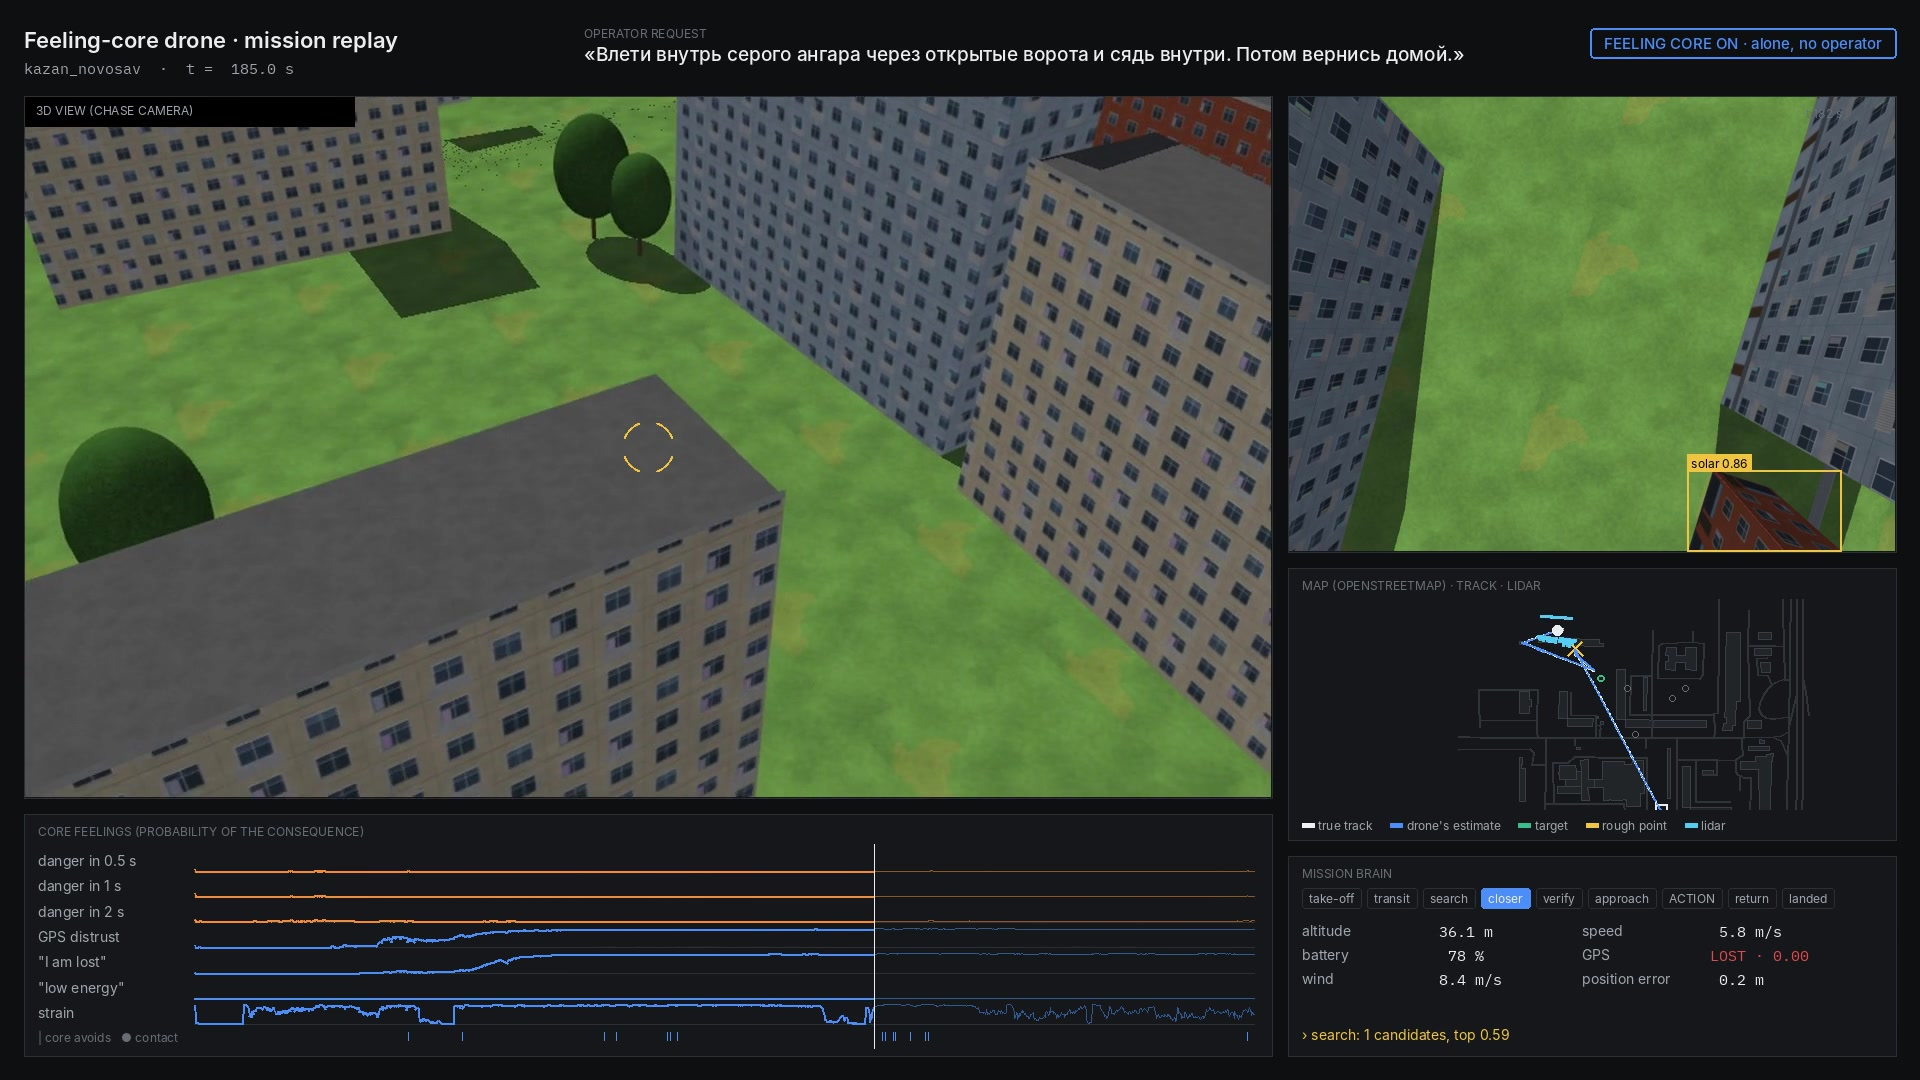
\includegraphics[width=\linewidth]{frame_mission_en.jpg}
\caption{One frame of mission G45 (enter a grey hangar, then return home) in the Kazan test district, 185\,s into the flight. GPS
was lost at 36\,s; the drone navigates on lidar and map, and its ``I am lost'' feeling has risen. Left: chase view, the core's
feelings over the whole flight, with the moments it overrode the brain. Right: the drone's camera with detections, the map with the
true track, the drone's own estimate and the rough point, and the mission brain's phase and state.}
\label{fig:frame}
\end{figure}

\begin{figure}[h]
\centering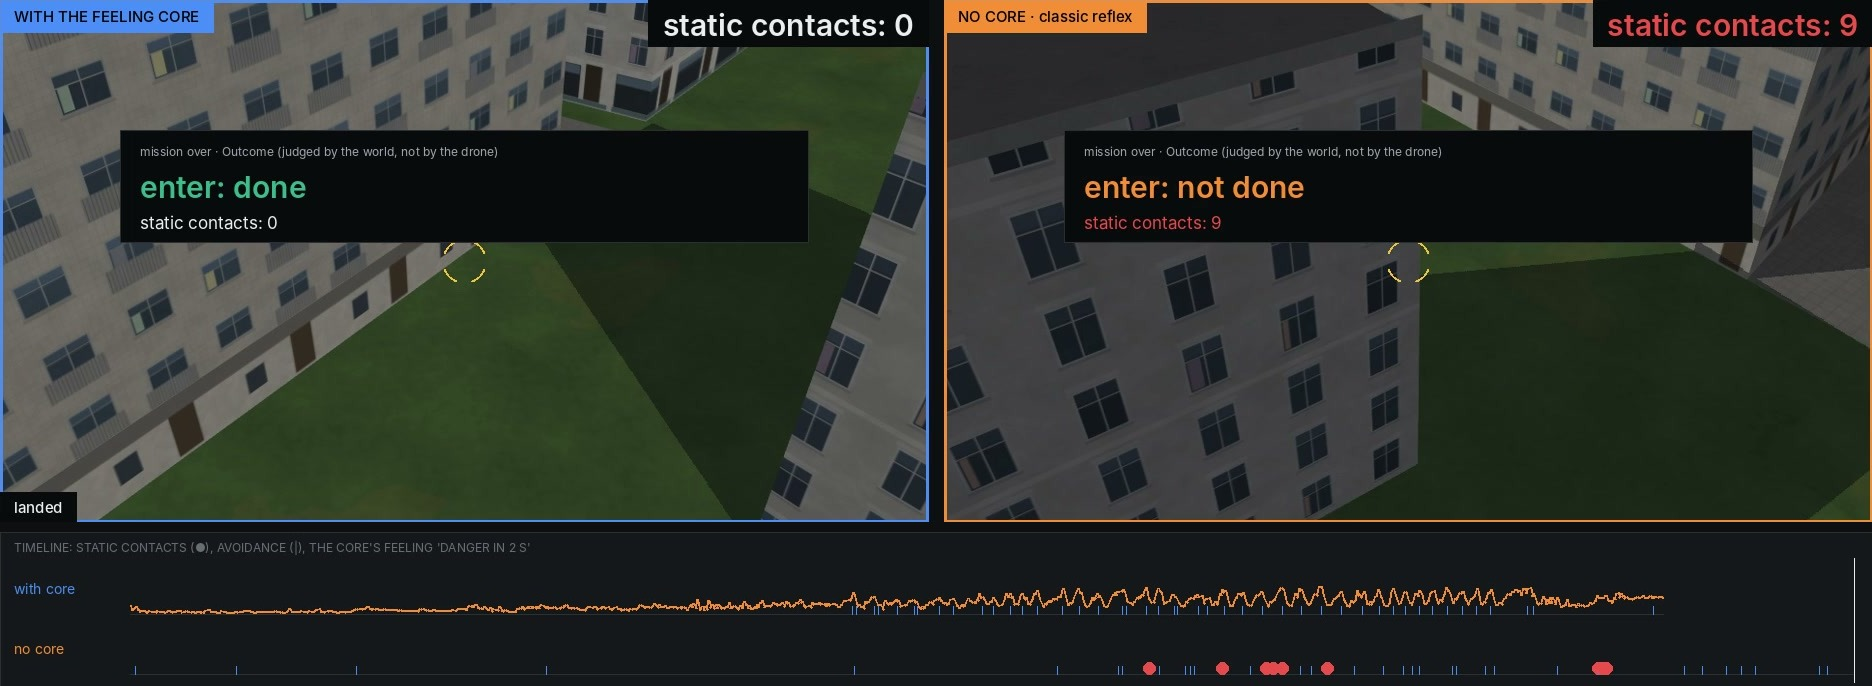
\includegraphics[width=\linewidth]{fig_compare_en.jpg}
\caption{One frame of the side-by-side video of mission G206 (enter a blue hangar, Tokyo test district): the same mission flown
with the feeling core (left) and with a classic reflex in its place (right), at the end of the mission. With the core the drone
entered the hangar without touching anything; with the reflex the entry failed after 9 static contacts. Bottom: the timeline of the
whole flight, with the static contacts of each drone (red dots) and the core's ``danger in 2\,s'' feeling. The four
side-by-side videos are replays of G2 missions run again from their plans on another GPU model; small numerical differences in the
detector change the course of a flight, so a replay differs in detail from the logged G2 flight. Over the four replays the core
had 1 static contact and the reflex 16; in one of them (G112) there was no difference, and in another (G45) the core failed the
hangar entry that the reflex made at the price of 6 contacts.}
\label{fig:compare}
\end{figure}

\begin{figure}[h]
\centering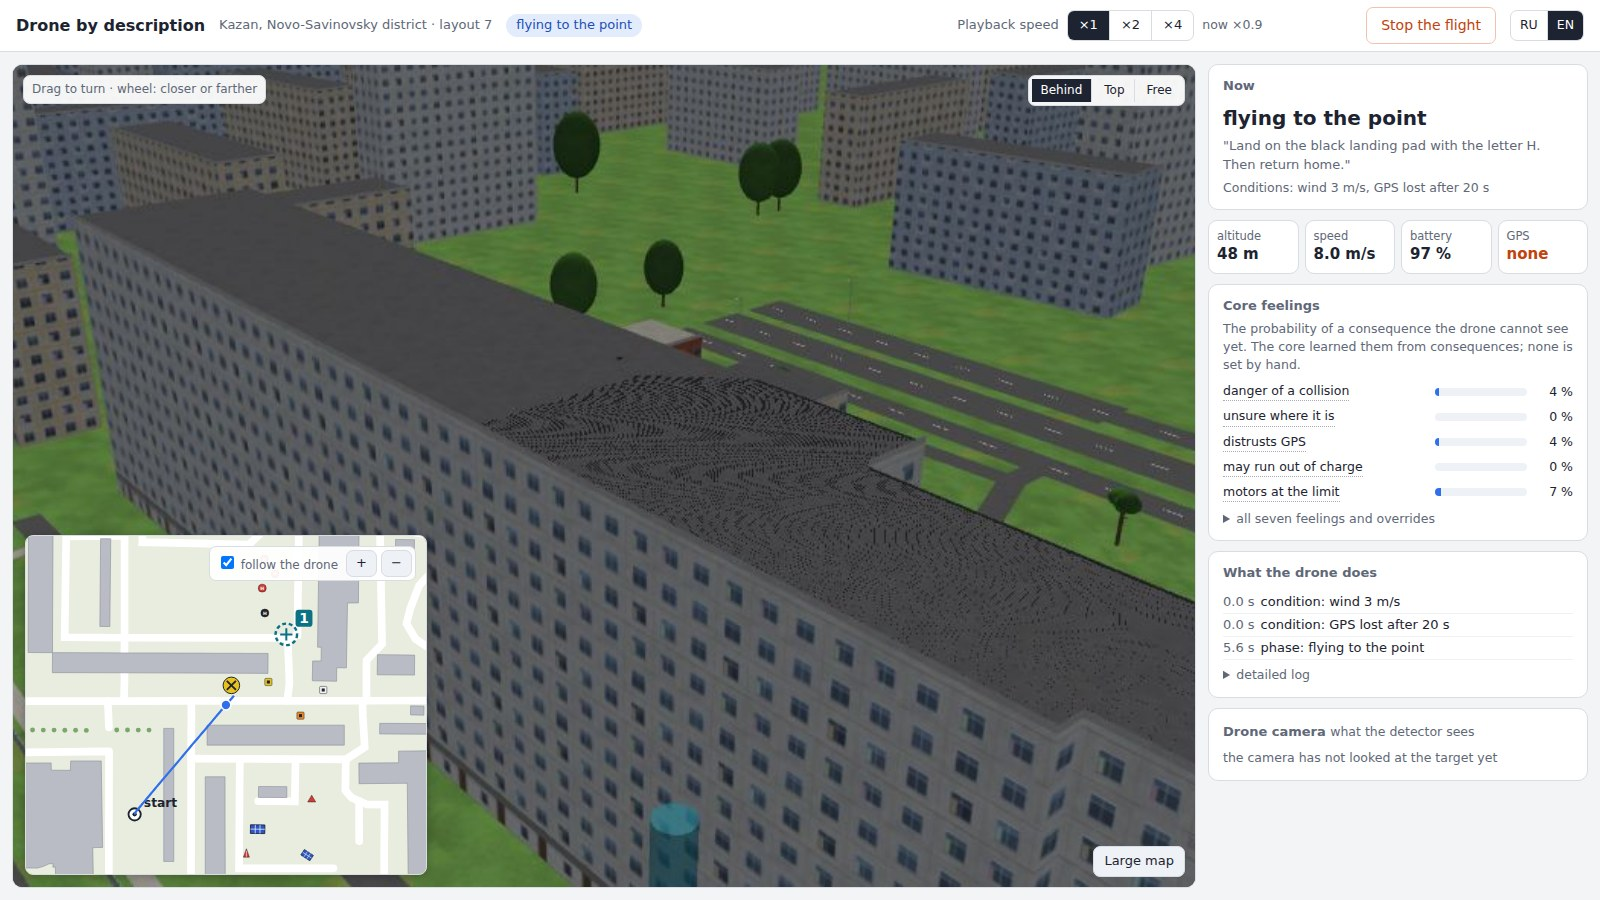
\includegraphics[width=\linewidth]{fig_app_en.jpg}
\caption{The app in flight (it has an English and a Russian interface). The large 3D chase view is rendered by the simulator itself; the map in
the corner shows the rough point, the true track and the drone's own estimate. On the right: the current phase, the conditions
(here GPS lost after 20\,s), altitude, speed, battery and GPS, five of the core's feelings and the event feed. Before the flight
the operator places a rough point, writes the request, checks the parse shown in plain words and picks the conditions.}
\label{fig:app}
\end{figure}

